\subsection{Flujo de caja}

El flujo de caja constituye una herramienta fundamental para la gestión financiera empresarial, permitiendo un seguimiento detallado de todos los movimientos de entrada y salida de dinero. Este análisis proporciona una perspectiva integral sobre la salud financiera de la organización, mostrando su capacidad para afrontar compromisos financieros, como pagos de deudas y otros gastos, en un periodo determinado.

La tabla \ref{flujoCaja} presenta de manera visual y detallada estos elementos financieros, facilitando así una mejor interpretación y evaluación de la situación económica de la empresa.

\vspace{2mm}
\begin{minipage}{0.8\textwidth}
\centering
\captionof{table}[{Flujo de caja }]{ Flujo de caja }
\label{flujoCaja}
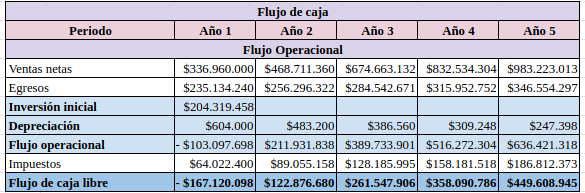
\includegraphics[width=0.9\textwidth]{Content/Images/AF/FlujoDeCaja.png}
\footnote{Nota. \textup{Fuente : Autores}}
\end{minipage}
\newpage